% !TeX root = ../main.tex
\documentclass[./../main.tex]{subfiles}

\begin{document}
Chương này gồm ba kiến thức nền tảng. Đầu tiên trình bày sơ bộ về các đối tượng và cách cấu trúc một tài liệu PDF, từ đó là bước đệm để hiểu cách phần mềm độc hại được nhúng vào tệp cũng như là cách để có thể xác định các bất thường trong cấu trúc một tệp PDF. Tiếp theo giới thiệu về một số thuật toán học máy được sử dụng khi xây dựng mô hình phân loại tự động các tệp PDF độc hại. Phần cuối cùng đưa ra cách tiếp cận và quy trình để có thể phát hiện tệp độc hại.

\section{Định dạng tài liệu PDF}
Hiện nay, PDF là một trong những định dạng phổ biến nhất để lưu trữ tài liệu trên toàn thế giới. Năm 1993, PDF được Adobe Systems định nghĩa và đến năm 2008, PDF đã trở thành một tiêu chuẩn mở được phát hành dưới chuẩn ISO 32000-1.

\subsection{Các đối tượng tài liệu}
Cấu trúc của tệp PDF bao gồm các đối tượng liên kết với nhau trong một cấu trúc cây. Những đối tượng này được chia thành ba loại, gồm có các đối tượng đơn giản, các đối tượng ghép và đối tượng độc lập.
\subsubsection*{Đối tượng đơn giản}
\begin{itemize}
	\item Boolean: lưu giá trị true/false.
	\item Number: là đối tượng số.
	\item String: là các xâu ký tự với kích thước tối đa 65535 bytes.
	\item Name: là các đối tượng từ khóa được định nghĩa sẵn trong tiêu chuẩn PDF, theo sau bởi ký tự '/', ví dụ '/kids' xác định các đối tượng con, '/filter' chỉ định bộ lọc được sử dụng,...
	\item Indirect reference: là các tham chiếu tới các đối tượng độc lập.
\end{itemize}
\subsubsection*{Đối tượng ghép}

\begin{itemize}
	\item Array: mảng 1 chiều các đối tượng được sắp xếp trong cặp ký tự '[]'.
	\item Dictionary: giống như một danh sách lưu trữ các cặp từ khóa - giá trị, được đặt trong cặp ký tự  '<<>>'. Từ khóa phải là một đối tượng Name còn giá trị thì có thể là bất kể đối tượng nào. Mỗi từ khóa chỉ xuất hiện 1 lần duy nhất trong một đối tượng dictionary.
	\item Stream: đối tượng stream giống như một đối tượng string, gồm một chuỗi các bytes, nhưng khác ở việc không giới hạn về độ dài. Do đó đối tượng stream có khả năng chứa một lượng lớn dữ liệu như hình ảnh, các thông tin mô tả trang,... Stream được đặt trong cặp từ khóa 'stream endstream'.
\end{itemize}
\subsubsection*{Đối tượng độc lập}

Các đối tượng độc lập có định danh là các cặp (number object, generation object) ứng với số hiệu đối tượng và thế hệ của đối tượng. Các đối tượng khác có thể tham chiếu tới qua định danh này. Các đối tượng độc lập được định nghĩa bên trong cặp từ khóa 'obj endobj'.




\subsection{Cấu trúc vật lý}
Cấu trúc vật lý của PDF xác định cách đối tượng được lưu trữ trong tệp, cách mà chúng được truy cập và cập nhật. Một tệp PDF cơ bản sẽ được xây dựng bằng bốn yếu tố: header, body, bảng tham chiếu xref table và trailer. Hình \ref{fig:initstruct} thể hiện cấu trúc này.

Cấu trúc ban đầu của PDF sẽ được thay đổi sau mỗi lần cập nhật, bằng cách thêm các sự thay đổi vào cuối của tệp, được gọi là cập nhật tăng dần.
% figure
\begin{figure}[ht!]
	\centering
	\includegraphics[width=0.5\linewidth]{./images/initial_structure.png}
	\caption{Cấu trúc vật lý của tệp PDF}
	\label{fig:initstruct}
\end{figure}

\subsubsection*{Header}
Header là dòng đầu tiên trong tệp PDF, xác định phiên bản tệp, được viết dưới định dạng '\%PDF-version'. Ví dụ '\%PDF-1.7' xác định phiên bản PDF hiện tại là 1.7.

Ngoài ra, nếu tệp PDF chứa dữ liệu nhị phân, header sẽ chứa một dòng comment gồm ít nhất 4 ký tự nhị phân giúp xác định được cần xử lý dữ liệu tệp dưới dạng văn bản hay nhị phân.

\subsubsection*{Body}
Phần body của tệp chứa tất cả các đối tượng lưu trữ những dữ liệu sẽ hiển thị cho người dùng, được xác định từ sau phần header đến khi xuất hiện từ khóa 'xref'. Những dữ liệu trong body sau đó có thể được chỉnh sửa, và phần cập nhật sẽ được lưu trữ ở cuối tệp.

\subsubsection*{Xref Table}
Xref table hay còn được gọi là cross-reference table là một bảng tham chiếu tới các đối tượng độc lập trong tài liệu nhằm mục đích cho phép truy cập ngẫu nhiên vào các đối tượng này mà không cần đọc toàn bộ tài liệu để định vị một đối tượng cụ thể.

Bảng có thể chứa một hoặc nhiều phần. Ban đầu, toàn bộ bảng chỉ bao gồm một phần duy nhất. Một phần tương ứng sẽ được thêm vào nếu tệp được thay đổi.
% figure
\begin{figure}[ht!]
	\centering
	\includegraphics[width=0.5\linewidth]{./images/xref_example.png}
	\caption{Một bảng xref trong tài liệu PDF}
	\label{fig:xreftable}
\end{figure}

Ở trên hình \ref{fig:xreftable}, cho thấy một ví dụ về bảng tham chiếu trong tệp PDF, gồm có 4 phần con, bắt đầu bởi dòng chứa hai giá trị số với giá trị đầu là số thứ tự của đối tượng đầu tiên, giá trị thứ hai là số lượng đối tượng trong phần con này. Ví dụ ở phần thứ 3, giá trị '21 4' cho thấy có 4 đối tượng trong phần con, được đánh số bắt đầu từ 21 đến 24. Theo sau đó là các dòng đại diện cho các đối tượng, xác định bởi một chuỗi gồm 20 byte lưu trữ địa chỉ của đối tượng (offset), số thế hệ của đối tượng và một cờ 'f' hoặc 'n. Cờ 'f' nghĩa là đối tượng vẫn tồn tại trong tệp nhưng được đánh dấu không nên được sử dụng, ngược lại, cờ 'n' xác định đối tượng đang được sử dụng.

\subsubsection*{Trailer}

Trailer PDF được lưu ở cuối tệp, chỉ định vị trí của bảng tham chiếu và các đối tượng đặc biệt khác, bắt đầu bởi từ khóa 'trailer' (Hình \ref{fig:trailer}).

% figure
\begin{figure}[ht!]
	\centering
	\includegraphics[width=0.7\linewidth]{./images/img_trailer_pdf.png}
	\caption{Một trailer trong tài liệu PDF}
	\label{fig:trailer}
\end{figure}

Trong đối tượng dictionary của trailer lưu trữ các giá trị:

\begin{itemize}
	\item Size: xác định số lượng đối tượng trong bảng tham chiếu (có đếm cả các đối tượng trong các phần mới cập nhật). Giá trị này phải là 1 số nguyên, và không thể là một đối tượng tham chiếu.
	\item Prev: xác định địa chỉ của bảng tham chiếu được cập nhật trước đó- được sử dụng khi có nhiều bảng tham chiếu.
	\item Root: tham chiếu tới một đối tượng gốc trong mô hình cấu trúc logic của PDF.
\end{itemize}


\subsubsection*{Cập nhật tăng dần}
PDF được thiết kế với khả năng cập nhật tăng dần, tức là có thể cập nhật bằng cách thêm các đối tượng thay đổi vào cuối tệp PDF mà không cần phải viết lại toàn bộ tệp, mục tiêu cập nhật nhanh chóng các thay đổi nhỏ vào trong 1 tệp lớn.

Có thể thấy trong hình \ref{fig:update}, tệp PDF vẫn chứa các phần header, body, xref table và trailer ban đầu. Tiếp theo sẽ có các body, xref table và trailer được thêm vào cuối tệp. Các bảng tham chiếu được bổ sung sẽ chỉ chứa các đối tượng đã bị thay đổi, thay thế  hoặc xóa. Các đối tượng bị xóa sẽ vẫn nằm trong tệp nhưng được đánh dấu với cờ 'f'.  Trong phần trailer được thêm mới sẽ có một cặp từ khóa '\textbackslash Prev' cho biết vị trí của bảng tham chiếu trước đó và cần phải kết thúc bằng ký tự kết thúc "\%\%EOF"
% figure
\begin{figure}[ht!]
	\centering
	\includegraphics[width=0.5\linewidth]{./images/img_increase_update.png}
	\caption{Cấu trúc tệp PDF khi có cập nhật }
	\label{fig:update}
\end{figure}
% \footnotetext{\url{https://www.iso.org/standard/51502.html}}
\subsection{Cấu trúc logic}

Cấu trúc logic của tài liệu PDF chỉ ra cách các đối tượng liên kết với nhau và được tổ chức sao cho các trình đọc PDF có thể hiểu và xử lý tài liệu một cách thích hợp. Các đối tượng này được xây dựng dựa trên một mô hình phân cấp dạng cây, với nút gốc là một đối tượng catalog (Hình \ref{fig:logic_structure}).

% figure
\begin{figure}[ht!]
	\centering
	\includegraphics[width=0.8\linewidth]{./images/logic_structure_pdf.png}
	\caption{Mô hình phân cấp các đối tượng bên trong cấu trúc logic của tài liệu PDF \protect\footnotemark}
	\label{fig:logic_structure}
\end{figure}

\footnotetext{\url{https://www.iso.org/standard/51502.html}}


\begin{description}
	\item[Catalog]  cung cấp thông tin chung về loại đối tượng nào sẽ được hiển thị trong tệp PDF, nội dung của tài liệu và một số hướng dẫn cụ thể cho các trình đọc PDF về cách hiển thị PDF lên màn hình sau khi được mở. Hình \ref{fig:catalog} là một ví dụ về một đối tượng catalog trong tệp PDF, với từ khóa 'PageMode' xác định cách tệp sẽ được hiển thị, 'OpenAction' chỉ định hành động sẽ được thực thi ngay sau khi mở tệp, và 'Pages' tham chiếu tới nút gốc của một cây các trang trong tài liệu PDF.
	      % figure
	      \begin{figure}[ht!]
		      \centering
		      \includegraphics[width=0.5\linewidth]{./images/catalog.png}
		      \caption{Đối tượng catalog trong tài liệu PDF}
		      \label{fig:catalog}
	      \end{figure}

	\item[Page Tree] Các trang của tài liệu PDF được liên kết thông qua một cây các trang - định nghĩa thứ tự truy cập. Sử dụng cấu trúc cây cho phép trình đọc nhanh chóng mở các trang trong tài liệu chứa hàng nghìn trang. Nút gốc của cây được chỉ định thông qua tham chiếu /Pages trong đối tượng Catalog.

\end{description}

\section{Một số thuật toán phân loại}

Ngoài việc hiểu cấu trúc tài liệu PDF phục vụ cho việc phân tích và trích xuất những đặc trưng có giá trị thì việc huấn luyện một bộ phân loại hai lớp để phát hiện các mẫu độc hại với độ chính xác cao nhất có thể là vô cùng quan trọng. Thông thường, những mô hình phân loại sẽ được áp dụng vào tập dữ liệu một cách độc lập, từ đó xem xét mô hình nào hoạt động tốt nhất. Ở phạm vi khóa luận này, một số thuật toán phân loại được sử dụng trong các thử nghiệm, bao gồm Cây quyết định, Random Forest và LightGBM.

\subsection{Cây quyết định}
Cây quyết định là một thuật toán học máy có giám sát được sử dụng rộng rãi. Một cây quyết định sử dụng mô hình cấu trúc cây để biểu thị các dự đoán xuất phát từ một loạt các điều kiện phân tách dựa trên các đặc trưng, bắt đầu với nút gốc và kết thúc bằng một quyết định đưa ra bởi nút lá (Hình \ref{fig:img_cart_01_gray}).

\begin{figure}[ht!]
	\centering
	\includegraphics[width=\linewidth]{./images/img_cart_01_gray.png}
	\caption{Sơ đồ cấu trúc cây trong thuật toán Cây quyết định}
	\label{fig:img_cart_01_gray}
\end{figure}

\begin{description}
	\item[Nút gốc] là nút bắt đầu của cây quyết định
	\item[Nút quyết định] các nút sau nút gốc, chứa những điều kiện để phân chia tới các nút tiếp theo.
	\item[Nút lá] nút kết thúc, chứa một nhãn duy nhất ứng với kết quả cuối cùng.
	\item[Cây con] là các phần nhỏ của đồ thị biểu diễn cây quyết định, theo sau bởi nút gốc hoặc một nút quyết định
\end{description}

Cây quyết định phân loại bằng cách duyệt mẫu từ trên xuống dưới bắt đầu từ gốc của cây, tại mỗi nút quyết định, điều kiện sẽ được kiểm tra và mẫu sẽ được phân phối xuống các nút tiếp theo, cho đến khi đến một nút lá. Nhãn của nút lá sẽ chính là kết quả phân loại cuối cùng cho mẫu đó.

Trên thực tế, thuật toán đã được sử dụng trong rất nhiều công bố về phân loại tệp PDF độc hại: Davide Maiorca và cộng sự \cite{davide}, Himanshu Pareek và cộng sự \cite{himanshu}. Ngoài ra một số công cụ phát hiện PDF độc hại như Hidost \cite{hidost}, Lux0R \cite{luxor} hay PDF Malware Slayer \cite{slayer} cũng sử dụng thuật toán này trong mô hình phân loại.

\subsection{Random Forest}

Random Forest là một thuật toán học kết hợp, bằng cách xây dựng rất nhiều các mô hình cây quyết định tạo thành rừng, mang lại một kết quả tốt hơn khi chỉ sử dụng một cây quyết định đơn lẻ. Mỗi cây quyết định trong rừng sẽ được học độc lập dựa trên một tập con ngẫu nhiên từ tập huấn luyện, và chỉ sử dụng một tập con các đặc trưng ngẫu nhiên của dữ liệu. Khi thực hiện phân loại, mẫu kiểm thử sẽ được phân loại song song trên các cây và trung bình cộng của các kết quả sẽ cho ra nhãn phân loại cuối cùng (Hình \ref{fig:img_rf_flow}).

\begin{figure}[ht!]
	\centering
	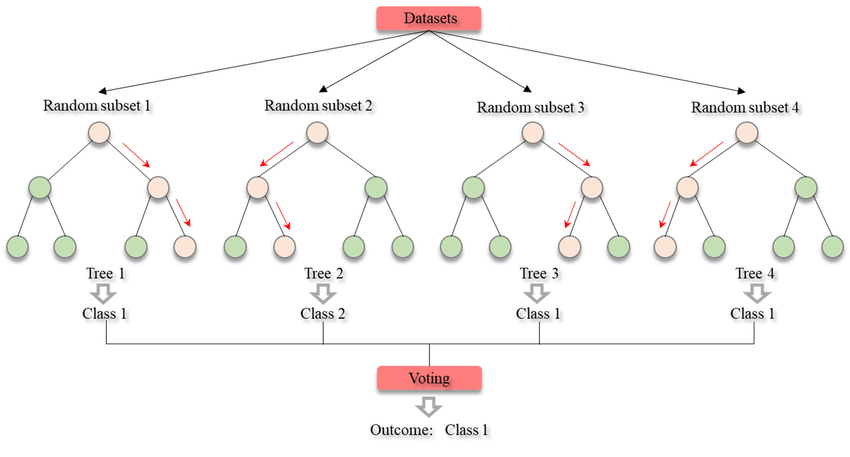
\includegraphics[width=\linewidth]{./images/img_rf_flow.png}
	\caption{Quy trình phân loại dựa trên thuật toán Random Forest \cite{randomforest}}
	\label{fig:img_rf_flow}
\end{figure}

Trong thuật toán Cây quyết định, khi xây dựng cây với một độ sâu tùy ý, có thể gây nên việc mô hình khớp hoàn toàn với dữ liệu tập huấn luyện, nhưng lại mang lại kết quả kém trên các tập kiểm thử (hiện tượng overfitting). Các cây trong thuật toán Random Forest chỉ dùng một phần dữ liệu huấn luyện để học, do đó sẽ không gặp overfitting nhưng có thể gây ra underfitting - khi số tập dữ liệu không đủ hoặc số lượng đặc trưng được sử dụng quá ít, dẫn tới kết quả xấu trên cả tập huấn luyện lẫn tập kiểm thử. Tuy nhiên, kết quả của thuật toán Random Forest là sự tổng hợp từ tất cả các cây quyết định, nhờ đó, các cây sẽ bổ sung cho nhau và mang lại một kết quả phân loại tốt hơn.

Thuật toán Random Forest đã được sử dụng trong các công cụ phát hiện mã độc như PDFRate \cite{pdfrate}, PDF Malware Slayer \cite{slayer} và LuxOR \cite{luxor}.

\subsection{Kỹ thuật boosting và thuật toán LightGBM}
Nhận thức được điểm yếu khi chỉ sử dụng một mô hình đơn lẻ như Cây quyết định, thuật toán Random Forest đưa ra một cải tiến mới khi kết hợp sử dụng mô hình trên nhiều phần dữ liệu khác nhau, huấn luyện độc lập và song song với nhau để đưa ra một kết quả tốt nhất. Đây là một ví dụ điển hình cho kỹ thuật bagging trong phương pháp học kết hợp. Ngoài ra, với phương pháp học kết hợp, một kỹ thuật được gọi là boosting cũng sẽ thực hiện xây dựng một chuỗi các mô hình trên những tập dữ liệu con khác nhau nhưng hoạt động học sẽ diễn ra một cách tuần tự. Theo đó, mô hình sau trong quá trình huấn luyện sẽ rút kinh nghiệm từ những lỗi của mô hình trước đó bằng cách cập nhật trọng số (Hình \ref{fig:compare_ensemble_methods}). Đầu ra của mô hình cuối cùng trong chuỗi sẽ là kết quả cuối cùng khi thực hiện phân loại.

\begin{figure}[ht!]
	\centering
	\includegraphics[width=\linewidth]{./images/compare_ensemble_methods.png}
	\caption{So sánh các kỹ thuật được sử dụng trong mô hình sử dụng phương pháp học kết hợp\protect\footnotemark}
	\label{fig:compare_ensemble_methods}
\end{figure}

\footnotetext{\url{https://mateusmaiads.github.io/ensemble_qualify}}

Trong phạm vi của khóa luận này, tôi đề xuất sử dụng một thuật toán boosting được phát triển bởi Microsoft là LightGBM \footnote{\url{https://lightgbm.readthedocs.io/en/v3.3.2/}}. LightGBM viết tắt của Light Gradient Boosting Machine, là một mô hình xử lý thuật toán học kết hợp tăng cường. Mô hình này cũng sử dụng Cây quyết định để xây dựng các mô hình thành phần. Sau mỗi lần thực hiện huấn luyện trên một mô hình với một tập dữ liệu con, thuật toán sẽ cập nhật tham số của mô hình theo hướng giảm của đạo hàm hàm mất mát.

Với nhiều kỹ thuật và cơ chế phức tạp, thuật toán LightGBM mang lại một bộ phân loại mạnh mẽ, tốc độ tính toán được tối ưu, do đó cần ít thời gian xử lý hơn so với các thuật toán cùng loại khác trên các tập huấn luyện có kích thước lớn \footnote{\url{https://lightgbm.readthedocs.io/en/v3.3.2/}}.

\section{Phát hiện tài liệu PDF độc hại}

Phát hiện các tệp độc hại có rất nhiều cách tiếp cận, tuy nhiên, có hai giai đoạn chính phục vụ mục đích này

\begin{itemize}
	\item Trích xuất đặc trưng
	\item Phân tích đặc trưng và đưa ra quyết định.
\end{itemize}


Trong giai đoạn trích xuất đặc trưng, các tệp PDF được xử lý và phân tích để trích xuất ra các đặc trưng cần thiết. Những đặc trưng này sẽ được thống kê và được đưa qua một bộ lọc để chọn ra những đặc trưng quan trọng trong giai đoạn Phân tích đặc trưng. Cuối cùng, một mô hình học máy sẽ được áp dụng để quyết định xem tệp đầu vào là sạch hay độc hại.

Mô hình \ref{fig:img5_tax} mô tả các đặc trưng được đề xuất để phát hiện tài liệu độc hại, và tổ chức chúng theo mô hình phân loại phân cấp. Mỗi cấp độ sẽ tương ứng với từng giai đoạn trong hoạt động trích xuất đặc trưng. Mô hình được giản lược từ mô hình được giới thiệu bởi Michele Elingiusti và cộng sự trong công bố năm 2018 \cite{tax}.

\begin{figure}[ht!]
	\centering
	\includegraphics[width=\linewidth]{./images/img5_tax.png}
	\caption{Phân loại các đặc trưng được sử dụng trong phát hiện tài liệu PDF độc hại}
	\label{fig:img5_tax}
\end{figure}


\subsection*{Loại dữ liệu}
Ở cấp đầu tiên, đại diện cho loại dữ liệu được trích xuất từ tài liệu PDF

\begin{itemize}
	\item Siêu dữ liệu (metadata) là tất cả những dữ liệu có thể được trích xuất từ dữ liệu “thô” của tệp PDF từ những mô tả, các mối liên hệ và cấu trúc bên trong tài liệu. Các siêu dữ liệu bao gồm các từ khóa xuất hiện trong tệp, số lượng các ký tự kết thúc tệp, tác giả, đường dẫn cấu trúc,...
	\item Embedded code gồm các đoạn mã hay các tệp được nhúng vào trong tài liệu PDF, có thể kể đến một số tệp thực thi hay một số mã shellcode, điển hình và xuất hiện nhiều nhất là các mã JavaScript.
\end{itemize}


\subsection*{Tiền xử lý}
Tiền xử lý cho thấy các kỹ thuật xử lý được sử dụng ứng với từng loại dữ liệu đầu vào, phục vụ cho mục đích cụ thể là đưa ra những đặc trưng hữu ích trong việc phát hiện tài liệu độc hại. Kết quả của quá trình xử lý này là một tập các đặc trưng - được liệt kê ở cấp cuối cùng. Các đặc trưng này sẽ là đầu vào của các mô hình học máy khi thực hiện phân loại tệp độc hại.

\begin{itemize}
	\item Phân tích cấu trúc của tệp PDF nhằm mục tiêu trích xuất các đặc trưng thống kê như từ khóa hay đường dẫn cấu trúc.
	\item Tham chiếu API mã JavaScript:  Quá trình xử lý và nhận diện các API được sử dụng trong mã JavaScript, bằng phương pháp phân tích tĩnh hoặc phân tích động. Cách tiếp cận này đã được đề xuất trong LuxOr \cite{luxor}. Đầu ra của quá trình này là các mẫu API được sử dụng nhiều trong các tài liệu độc hại hay các tài liệu lành tính.
	\item Phân tích từ vựng: các đoạn mã JavaScript thường bị xáo trộn và làm phức tạp hóa, điều này yêu cầu một dạng biểu diễn trừu tượng hóa để loại bỏ các chi tiết không cần thiết và cô lập những đoạn mã thực sự liên quan để dễ dàng trong việc nhận diện và phát hiện bất thường. Một quy trình phân tích từ vựng mã nguồn sẽ hỗ trợ tự động hóa quá trình trừu tượng hóa như vậy. Cách tiếp cận này đã được đề xuất bởi Vatamanu và cộng sự \cite{vatamanu} sử dụng công cụ SpiderMonkey \footnote{\url{https://spidermonkey.dev/}} để trích xuất ra các JavaScript token.
	\item Trích xuất opcode: một kỹ thuật tấn công được sử dụng trong các tài liệu PDF độc hại là xây dựng các đoạn mã shellcode trong thời gian thực thi bằng cách sao chép các chuỗi opcode ẩn giấu trong các biến. Do đó, một phương pháp phát hiện được đề xuất thực hiện phân tích động để xác định các biến có thể chứa các chuỗi opcode độc hại hoặc đáng ngờ. PDF Scrutinizer \cite{scrutinizer} xây dựng một phương pháp phỏng đoán đề xác định vị trí nào cần để phân tích. MDScan \cite{mdscan} chọn các chuỗi cần tìm shellcode bằng cách quan sát các chuỗi được tạo ra trong thời gian chạy, quét các vùng nhớ của các chuỗi mới được cấp phát.

\end{itemize}


\end{document}